\documentclass[journal,12pt,twocolumn]{IEEEtran}

\usepackage{setspace}
\usepackage{gensymb}
\singlespacing
\usepackage[cmex10]{amsmath}
\usepackage{amssymb}
\usepackage{xurl}
\usepackage{tabularx}
\usepackage{amsthm}
\usepackage{comment}
\usepackage{mathrsfs}
\usepackage{txfonts}
\usepackage{stfloats}
\usepackage{bm}
\usepackage{cite}
\usepackage{cases}
\usepackage{subfig}
\usepackage{amsmath}
\usepackage{longtable}
\usepackage{multirow}
\usepackage{multicol}

\usepackage{enumitem}
\usepackage{mathtools}
\usepackage{steinmetz}
\usepackage{tikz}
\usepackage{circuitikz}
\usepackage{verbatim}
\usepackage{tfrupee}
\usepackage[breaklinks=true]{hyperref}
\usepackage{graphicx}
\usepackage{tkz-euclide}

\usetikzlibrary{calc,math}
\usepackage{listings}
    \usepackage{color}                                            %%
    \usepackage{array}                                            %%
    \usepackage{longtable}                                        %%
    \usepackage{calc}                                             %%
    \usepackage{multirow}                                         %%
    \usepackage{hhline}                                           %%
    \usepackage{ifthen}                                           %%
    \usepackage{lscape}     
\usepackage{multicol}
\usepackage{chngcntr}

\DeclareMathOperator*{\Res}{Res}

\renewcommand\thesection{\arabic{section}}
\renewcommand\thesubsection{\thesection.\arabic{subsection}}
\renewcommand\thesubsubsection{\thesubsection.\arabic{subsubsection}}

\renewcommand\thesectiondis{\arabic{section}}
\renewcommand\thesubsectiondis{\thesectiondis.\arabic{subsection}}
\renewcommand\thesubsubsectiondis{\thesubsectiondis.\arabic{subsubsection}}


\hyphenation{op-tical net-works semi-conduc-tor}
\def\inputGnumericTable{}                                 %%

\lstset{
%language=C,
frame=single, 
breaklines=true,
columns=fullflexible
}
\begin{document}


\newtheorem{theorem}{Theorem}[section]
\newtheorem{problem}{Problem}
\newtheorem{proposition}{Proposition}[section]
\newtheorem{lemma}{Lemma}[section]
\newtheorem{corollary}[theorem]{Corollary}
\newtheorem{example}{Example}[section]
\newtheorem{definition}[problem]{Definition}

\newcommand{\BEQA}{\begin{eqnarray}}
\newcommand{\EEQA}{\end{eqnarray}}
\newcommand{\define}{\stackrel{\triangle}{=}}
\bibliographystyle{IEEEtran}
\raggedbottom
\setlength{\parindent}{0pt}
\providecommand{\mbf}{\mathbf}
\providecommand{\pr}[1]{\ensuremath{\Pr\left(#1\right)}}
\providecommand{\qfunc}[1]{\ensuremath{Q\left(#1\right)}}
\providecommand{\sbrak}[1]{\ensuremath{{}\left[#1\right]}}
\providecommand{\lsbrak}[1]{\ensuremath{{}\left[#1\right.}}
\providecommand{\rsbrak}[1]{\ensuremath{{}\left.#1\right]}}
\providecommand{\brak}[1]{\ensuremath{\left(#1\right)}}
\providecommand{\lbrak}[1]{\ensuremath{\left(#1\right.}}
\providecommand{\rbrak}[1]{\ensuremath{\left.#1\right)}}
\providecommand{\cbrak}[1]{\ensuremath{\left\{#1\right\}}}
\providecommand{\lcbrak}[1]{\ensuremath{\left\{#1\right.}}
\providecommand{\rcbrak}[1]{\ensuremath{\left.#1\right\}}}
\theoremstyle{remark}
\newtheorem{rem}{Remark}
\newcommand{\sgn}{\mathop{\mathrm{sgn}}}
\providecommand{\abs}[1]{\vert#1\vert}
\providecommand{\res}[1]{\Res\displaylimits_{#1}} 
\providecommand{\norm}[1]{\lVert#1\rVert}
%\providecommand{\norm}[1]{\lVert#1\rVert}
\providecommand{\mtx}[1]{\mathbf{#1}}
\providecommand{\mean}[1]{E[ #1 ]}
\providecommand{\fourier}{\overset{\mathcal{F}}{ \rightleftharpoons}}
%\providecommand{\hilbert}{\overset{\mathcal{H}}{ \rightleftharpoons}}
\providecommand{\system}{\overset{\mathcal{H}}{ \longleftrightarrow}}
	%\newcommand{\solution}[2]{\textbf{Solution:}{#1}}
\newcommand{\solution}{\noindent \textbf{Solution: }}
\newcommand{\cosec}{\,\text{cosec}\,}
\providecommand{\dec}[2]{\ensuremath{\overset{#1}{\underset{#2}{\gtrless}}}}
\newcommand{\myvec}[1]{\ensuremath{\begin{pmatrix}#1\end{pmatrix}}}
\newcommand{\mydet}[1]{\ensuremath{\begin{vmatrix}#1\end{vmatrix}}}
\newcommand*{\permcomb}[4][0mu]{{{}^{#3}\mkern#1#2_{#4}}}
\newcommand*{\perm}[1][-3mu]{\permcomb[#1]{P}}
\newcommand*{\comb}[1][-1mu]{\permcomb[#1]{C}}
\numberwithin{equation}{subsection}
\makeatletter
\@addtoreset{figure}{problem}
\makeatother
\let\StandardTheFigure\thefigure
\let\vec\mathbf
\renewcommand{\thefigure}{\theproblem}
\def\putbox#1#2#3{\makebox[0in][l]{\makebox[#1][l]{}\raisebox{\baselineskip}[0in][0in]{\raisebox{#2}[0in][0in]{#3}}}}
     \def\rightbox#1{\makebox[0in][r]{#1}}
     \def\centbox#1{\makebox[0in]{#1}}
     \def\topbox#1{\raisebox{-\baselineskip}[0in][0in]{#1}}
     \def\midbox#1{\raisebox{-0.5\baselineskip}[0in][0in]{#1}}
\vspace{3cm}
\title{Assignment 2}
\author{CS20BTECH11047}
\maketitle
\newpage
\bigskip
\renewcommand{\thefigure}{\arabic{figure}}
\renewcommand{\thetable}{\arabic{table}}
Download all python codes from 
\begin{lstlisting}
https://github.com/JeevanIITH/AI1102/blob/main/assignment2/assignment2.py
\end{lstlisting}
%
and latex codes from 
%
\begin{lstlisting}
https://github.com/JeevanIITH/AI1102/blob/main/assignment2/assignment2.tex
\end{lstlisting}
\section*{section}
Let X and Y be two continuous random variables with the joint probability density function\\
\begin{align}
    f\left(x,y\right)=\begin{cases}
    2 \quad  0<x+y<1 ,x>0 ,y>0\\
    0 \quad  \textrm{elsewhere}\\
    \end{cases}
\end{align}
\\
Then $P\left(X+Y<\dfrac{1}{2}\right)$ is\\
%$\begin{align}
  \begin{multicols}{2}
   \begin{enumerate}
   
     \item $\dfrac{1}{4}$\\
     \item $\dfrac{1}{2}$\\
     \item $\dfrac{3}{4}$\\
     \item  1\\
   \end{enumerate}
   \end{multicols}
%\end{align}
%Then $P\left(X+Y<\dfrac{1}{2}\right)$ is \\
%1) $\dfrac{1}{4}$  \quad \quad 3) $\dfrac{3}{4}$\\
%\\
%2) $\dfrac{1}{2}$  \quad \quad  4) $1$
\section*{Solution}
Given X and Y be two continuous random variables with the joint probability density function
\begin{align}
    f\left(x,y\right)=\begin{cases}
    2 \quad  0<x+y<1 ,x>0 ,y>0\\
    0 \quad  \textrm{elsewhere}\\
    \end{cases}
\end{align}
\begin{figure}[h]
    \centering
    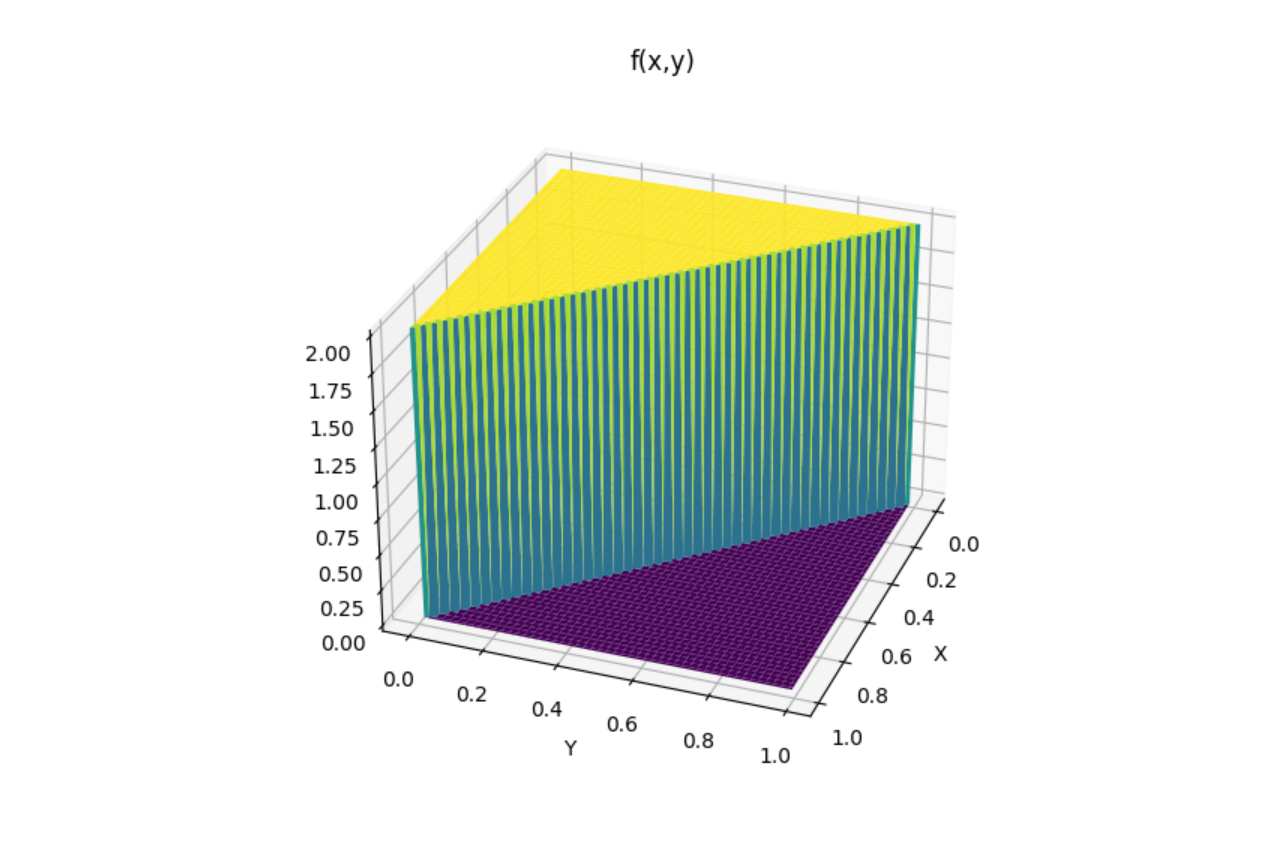
\includegraphics[scale=0.2]{f(x,y)_graph.png}
    \caption{$f\left(x,y\right)$}
    \label{fig:f(x,y)}
\end{figure}

we know that
\begin{align}
    P\left(\left(x,y\right)\in A\right)=\int \int _{A}f\left(x,y\right) dx dy \quad  A \in \mathbb{R}^2
\end{align}
from given information\\
for positive $x$ and $y$
\begin{align}
    0<x+y<\dfrac{1}{2}  \Rightarrow 0<x<\dfrac{1}{2}-y
\end{align}
so using eq(0.0.3)
\begin{align}
    P\left(x+y < \dfrac{1}{2}\right)=\int_{0}^{\frac{1}{2}} \int _{0}^{\frac{1}{2}-y}f(x,y) dx dy\\
    =\int_{0}^{\frac{1}{2}} \int _{0}^{\frac{1}{2}-y} 2 \quad dx dy
    =\int_{0}^{\frac{1}{2}} \left(  2 x \quad \big|_{0}^{\frac{1}{2}-y} \right)  dy\\
    =\int_{0}^{\frac{1}{2}}   2 \left(\frac{1}{2}-y\right) \quad    dy
    =2\left( \frac{1}{2} y - \frac{y^2}{2}  \right) \big|_{0}^{\frac{1}{2}}\\
    = \left( \frac{1}{2} - \frac{1}{4}\right) = \frac{1}{4} 
\end{align}
Therefore 
\begin{align}
    P\left(X+Y<\dfrac{1}{2}\right)=\dfrac{1}{4}
\end{align}
\begin{align}
\intertext{volume under the graph which contains the region} X+Y<\dfrac{1}{2} \quad \text{gives us} \quad P\left(X+Y<\dfrac{1}{2}\right) \\
 P\left(X+Y<\dfrac{1}{2}\right)= \text{Area of the base . height}
 \end{align}
 
Area of the base triangle is 
\begin{align}
 \dfrac{1}{2}.\textit{height}.\textit{base} =\dfrac{1}{2}.\dfrac{1}{2}.\dfrac{1}{2}
 \end{align}
 \begin{align}
\text{volume = Area . height}=\dfrac{1}{8}. 2= \dfrac{1}{4}
\end{align}
%The volume under the graph which contains the region $X+Y<\dfrac{1}{2}$ %gives us $P\left(x+y<\dfrac{1}{2}\right)$\\
%$P\left(x+y<\dfrac{1}{2}\right)=$ Area of the base . height\\
%Area of the base triangle is $\dfrac{1}{2}.\textit{height}.\textit{base}$%$= \dfrac{1}{2}.\dfrac{1}{2}.\dfrac{1}{2}$\\
%volume = Area . height $= \dfrac{1}{8}. 2= \dfrac{1}{4}$

\begin{figure}[h]
    \centering
    %\columnwidth
    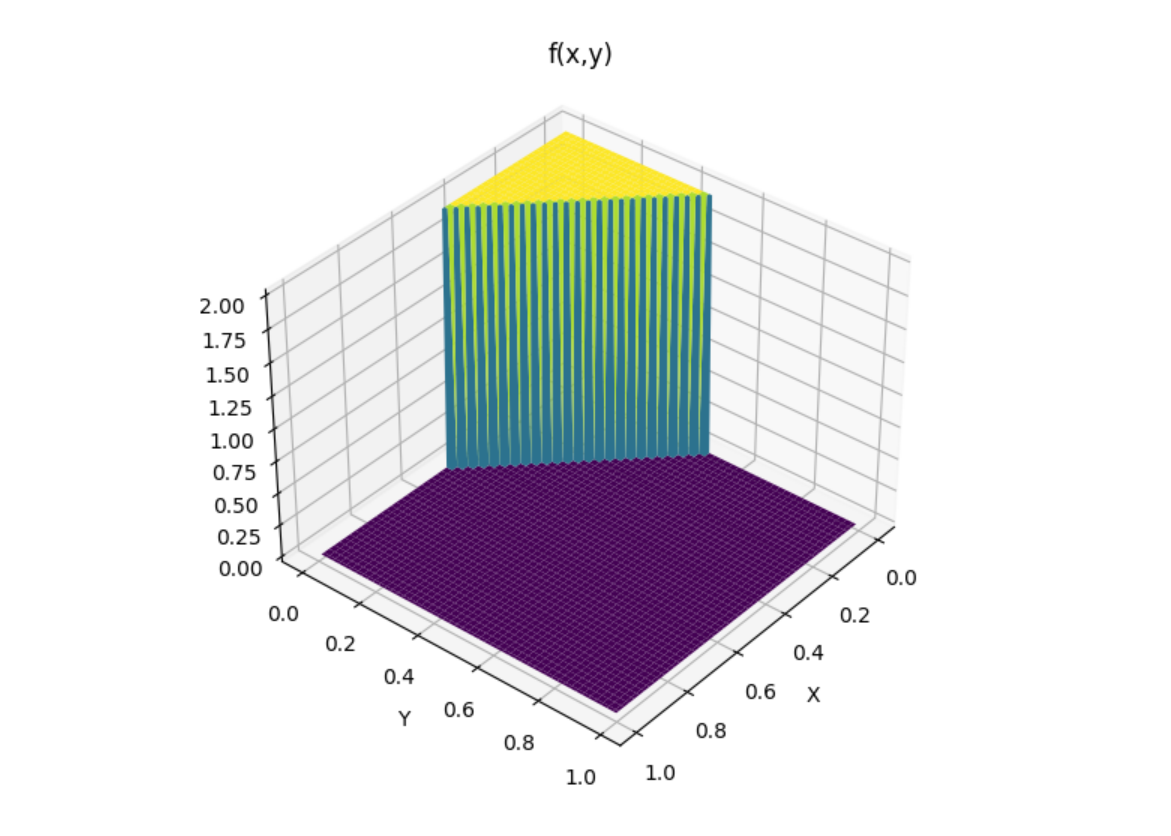
\includegraphics[width=\columnwidth]{P(x+y_2)_graph.png}
    \caption{$P\left(x+y<\dfrac{1}{2}\right)$}
    \label{fig:p(x+y<1/2)}
\end{figure}

\end{document}
